\documentclass[aspectratio=169]{beamer}

% ── Packages ────────────────────────────────────────────────────────────────
\usepackage[T1]{fontenc}
\usepackage[utf8]{inputenc}
\usepackage{lmodern}
\usepackage{microtype}
\usepackage{xcolor}
\usepackage{tikz}
\usepackage{booktabs}
\usepackage{fontawesome5}
\usepackage{array}
\usepackage{setspace}

% ── WUR colour palette ───────────────────────────────────────────────────────
\definecolor{wurgreen}{HTML}{34B233}
\definecolor{darkgreen}{HTML}{1F6B1E}
\definecolor{lightgreen}{HTML}{E8F7E8}
\definecolor{darknavy}{HTML}{1A1A2E}
\definecolor{midgray}{HTML}{6B7280}
\definecolor{lightgray}{HTML}{F3F4F6}
\definecolor{bodytext}{HTML}{1F2937}

% ── Beamer theme ────────────────────────────────────────────────────────────
\usetheme{default}
\usecolortheme{default}
\usefonttheme{professionalfonts}
\setbeamertemplate{navigation symbols}{}
\setbeamertemplate{itemize items}{\textcolor{wurgreen}{\textbullet}}
\setbeamertemplate{itemize subitem}{\textcolor{midgray}{--}}

% Frametitle
\setbeamercolor{frametitle}{fg=white, bg=darknavy}
\setbeamertemplate{frametitle}{%
  \begin{beamercolorbox}[wd=\paperwidth, ht=1.1cm, dp=0.2cm, leftskip=0.6cm]{frametitle}
    \usebeamerfont{frametitle}\insertframetitle
  \end{beamercolorbox}%
}
\setbeamerfont{frametitle}{size=\large, series=\bfseries}

% Background
\setbeamercolor{background canvas}{bg=white}
\setbeamercolor{normal text}{fg=bodytext}
\setbeamerfont{normal text}{size=\small}

% Footer
\setbeamertemplate{footline}{%
  \begin{beamercolorbox}[wd=\paperwidth, ht=0.4cm, dp=0.15cm]{footline}%
    \hspace{0.5cm}%
    \textcolor{midgray}{\tiny Bags, Vectors \& Transformers · Wageningen University \& Research}%
    \hfill%
    \textcolor{midgray}{\tiny \insertframenumber}%
    \hspace{0.4cm}%
  \end{beamercolorbox}%
}

% ── Helper: section block ────────────────────────────────────────────────────
\newcommand{\wurblock}[3]{%
  % #1 bg color, #2 fg color, #3 content
  \begin{tikzpicture}
    \node[fill=#1, text=#2, rounded corners=2pt,
          inner xsep=8pt, inner ysep=6pt, text width=\linewidth-22pt]{#3};
  \end{tikzpicture}%
}

% ── Title slide setup ────────────────────────────────────────────────────────
\title{Bags, Vectors \& Transformers}
\subtitle{A Methods Workshop in Computational Text Analysis}
\author{Denise J. Roth}
\institute{Strategic Communication Group\\Wageningen University \& Research}
\date{Autumn 2026}

% ════════════════════════════════════════════════════════════════════════════
\begin{document}
% ════════════════════════════════════════════════════════════════════════════

% ── PART I TITLE SLIDE ───────────────────────────────────────────────────────
{
\setbeamertemplate{footline}{}
\begin{frame}[plain]
  \begin{tikzpicture}[remember picture, overlay]
    \fill[darknavy] (current page.south west) rectangle (current page.north east);
    \fill[wurgreen] (current page.south west) rectangle
      ([xshift=0.45cm]current page.north west);
    \node[anchor=west, text=white, font=\huge\bfseries, text width=13cm]
      at ([xshift=1.1cm, yshift=1.2cm]current page.west)
      {Bags, Vectors \& Transformers};
    \node[anchor=west, text=wurgreen, font=\large, text width=12cm]
      at ([xshift=1.1cm, yshift=0.05cm]current page.west)
      {Introduction · Day 1, Part 1};
    \node[anchor=west, text=midgray, font=\small, text width=12cm]
      at ([xshift=1.1cm, yshift=-1.5cm]current page.west)
      {Denise J. Roth, PhD Candidate\\
       Strategic Communication Group · Wageningen University \& Research};
  \end{tikzpicture}
\end{frame}
}

% ── SLIDE 2: Agenda ──────────────────────────────────────────────────────────
\begin{frame}{Today's Session}
\vspace{0.2cm}
\begin{columns}[t]
  \column{0.5\textwidth}
    \medskip
    \textcolor{wurgreen}{\faHandPaper}\enspace \textbf{Welcome \& Introductions}\\
    {\small\textcolor{midgray}{Who we are --- and who you are}}

    \bigskip
    \textcolor{wurgreen}{\faSearch}\enspace \textbf{What is Computational Text Analysis?}\\
    {\small\textcolor{midgray}{The big picture}}

    \bigskip
    \textcolor{wurgreen}{\faLightbulb}\enspace \textbf{Why Should You Care?}\\
    {\small\textcolor{midgray}{Research examples and possibilities}}

  \column{0.5\textwidth}
    \medskip
    \textcolor{wurgreen}{\faBullseye}\enspace \textbf{What Could This Mean for Your Research?}\\
    {\small\textcolor{midgray}{Your data, your questions}}

    \bigskip
    \textcolor{wurgreen}{\faCalendar}\enspace \textbf{Course Overview}\\
    {\small\textcolor{midgray}{The 4-day journey ahead}}

    \bigskip
    \textcolor{wurgreen}{\faClipboard}\enspace \textbf{Practicalities}\\
    {\small\textcolor{midgray}{Tools, schedule, and expectations}}
\end{columns}
\end{frame}

% ── SLIDE 3: Meet your instructor ────────────────────────────────────────────
\begin{frame}{Meet Your Instructor}
\vspace{0.2cm}
\begin{columns}[c]
  \column{0.22\textwidth}
    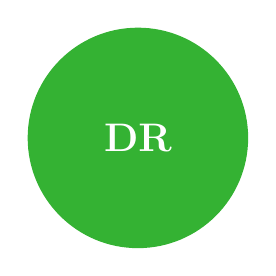
\begin{tikzpicture}
      \fill[wurgreen] (0,0) circle (1.4cm);
      \node[text=white, font=\Large\bfseries] at (0,0) {DR};
    \end{tikzpicture}

  \column{0.75\textwidth}
    {\large\textbf{Denise J. Roth}}\\[2pt]
    {\small\textcolor{midgray}{PhD Candidate \textperiodcentered\
     Strategic Communication Group\\
     Wageningen University \& Research}}

    \bigskip
    \begin{itemize}\setlength\itemsep{6pt}
      \item[\textcolor{wurgreen}{\faCompass}]
        Online political communication --- incivility, polarization, public discourse
      \item[\textcolor{wurgreen}{\faSearch}]
        Black digital health communication and scientization of public debate
      \item[\textcolor{wurgreen}{\faPython}]
        Computational text analysis as a method across all of the above
    \end{itemize}

    \bigskip
    {\small\textit{\textcolor{midgray}{Feel free to ask questions throughout --- this is a participatory course!}}}
\end{columns}
\end{frame}

% ── SLIDE 4: Student introductions ───────────────────────────────────────────
\begin{frame}{Now You! \faHandPaper}
\vspace{0.15cm}
{\small Take a moment to introduce yourself to the group:}

\bigskip
\begin{tikzpicture}
  \node[fill=lightgreen, draw=wurgreen, rounded corners=3pt,
        inner xsep=10pt, inner ysep=7pt, text width=\textwidth-26pt]{%
    \textcolor{wurgreen}{\faUser}\enspace Your name and department};
\end{tikzpicture}

\smallskip

\begin{tikzpicture}
  \node[fill=lightgray, rounded corners=3pt,
        inner xsep=10pt, inner ysep=7pt, text width=\textwidth-26pt]{%
    \textcolor{wurgreen}{\faMicroscope}\enspace What you are researching};
\end{tikzpicture}

\smallskip
\begin{tikzpicture}
  \node[fill=lightgreen, draw=wurgreen, rounded corners=3pt,
        inner xsep=10pt, inner ysep=7pt, text width=\textwidth-26pt]{%
    \textcolor{wurgreen}{\faFile}\enspace What kind of text data you work with (or wish you could)};
\end{tikzpicture}

\smallskip

\begin{tikzpicture}
  \node[fill=lightgray, rounded corners=3pt,
        inner xsep=10pt, inner ysep=7pt, text width=\textwidth-26pt]{%
    \textcolor{wurgreen}{\faCog}\enspace Prior experience with methods or software (R, Python, SPSS\ldots\ anything!)};
\end{tikzpicture}

\smallskip
\begin{tikzpicture}
  \node[fill=lightgreen, draw=wurgreen, rounded corners=3pt,
        inner xsep=10pt, inner ysep=7pt, text width=\textwidth-26pt]{%
    \textcolor{wurgreen}{\faCompass}\enspace One thing you hope to get out of this course};
\end{tikzpicture}
\end{frame}

% ── SLIDE 5: What is CTA? ────────────────────────────────────────────────────
\begin{frame}{What is Computational Text Analysis?}
\vspace{0.15cm}
{\small\textit{Using computers to systematically extract patterns and meaning from large collections of text --- at a scale no human reader could manage alone.}}

\medskip
\begin{columns}[t]
  \column{0.48\textwidth}
    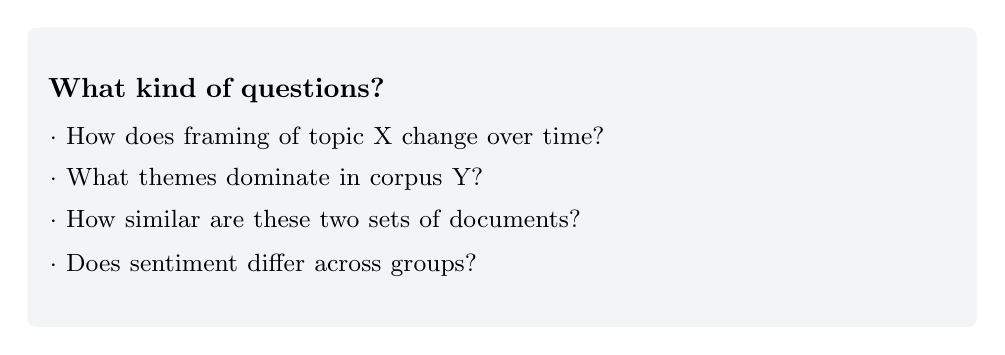
\begin{tikzpicture}
      \node[fill=lightgray, rounded corners=3pt,
            inner xsep=8pt, inner ysep=8pt, text width=\columnwidth-18pt, minimum height=3.8cm, anchor=north west]{%
        \textbf{What kind of questions?}\\[6pt]
        {\small
        $\cdot$ How does framing of topic X change over time?\\[4pt]
        $\cdot$ What themes dominate in corpus Y?\\[4pt]
        $\cdot$ How similar are these two sets of documents?\\[4pt]
        $\cdot$ Does sentiment differ across groups?}};
    \end{tikzpicture}

  \column{0.48\textwidth}
    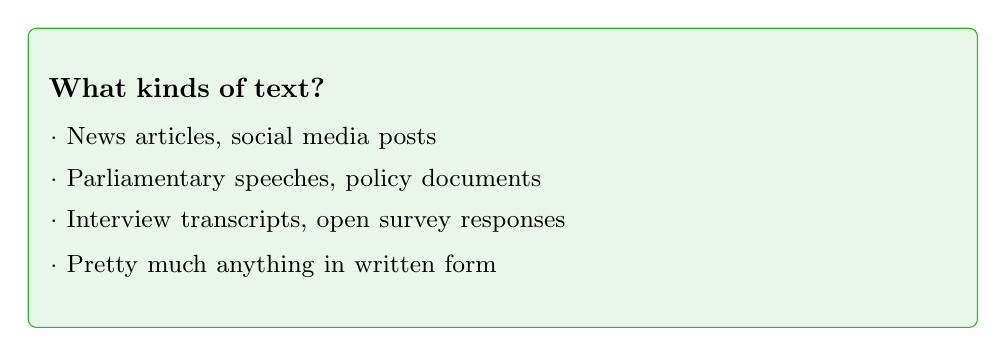
\begin{tikzpicture}
      \node[fill=lightgreen, draw=wurgreen, rounded corners=3pt,
            inner xsep=8pt, inner ysep=8pt, text width=\columnwidth-18pt, minimum height=3.8cm, anchor=north west]{%
        \textbf{What kinds of text?}\\[6pt]
        {\small
        $\cdot$ News articles, social media posts\\[4pt]
        $\cdot$ Parliamentary speeches, policy documents\\[4pt]
        $\cdot$ Interview transcripts, open survey responses\\[4pt]
        $\cdot$ Pretty much anything in written form}};
    \end{tikzpicture}
\end{columns}

\medskip
{\small\textcolor{midgray}{\textit{The method is flexible --- what matters is having a research question text can answer.}}}
\end{frame}

% ── SLIDE 5b: Quant or qual? ─────────────────────────────────────────────────
\begin{frame}{Quantitative or Qualitative?}
\vspace{0.1cm}
{\small\textit{Spoiler: it's both --- and that's what makes it powerful.}}

\bigskip
\begin{columns}[t]
  \column{0.31\textwidth}
    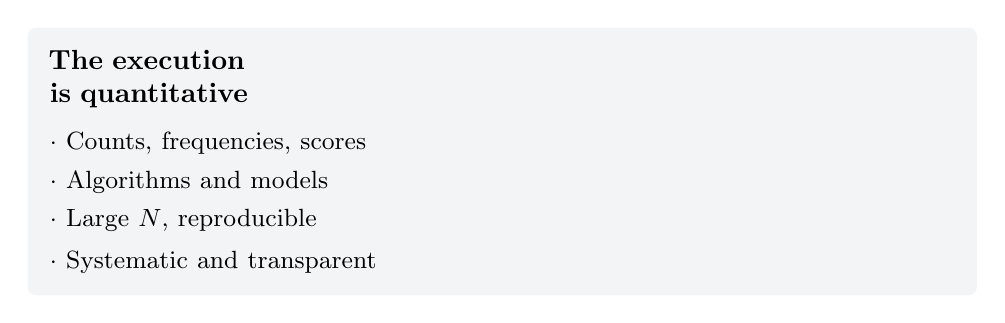
\begin{tikzpicture}
      \node[fill=lightgray, rounded corners=3pt,
            inner xsep=8pt, inner ysep=8pt, text width=\columnwidth-18pt]{%
        \textbf{The execution\\is quantitative}\\[6pt]
        {\small
        $\cdot$ Counts, frequencies, scores\\[3pt]
        $\cdot$ Algorithms and models\\[3pt]
        $\cdot$ Large $N$, reproducible\\[3pt]
        $\cdot$ Systematic and transparent}};
    \end{tikzpicture}

  \column{0.31\textwidth}
    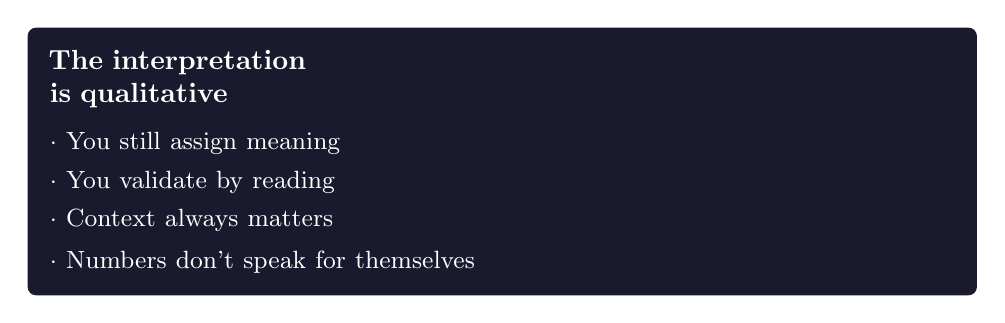
\begin{tikzpicture}
      \node[fill=darknavy, rounded corners=3pt,
            inner xsep=8pt, inner ysep=8pt, text width=\columnwidth-18pt]{%
        \textcolor{white}{\textbf{The interpretation\\is qualitative}}\\[6pt]
        {\small\textcolor{white}{
        $\cdot$ You still assign meaning\\[3pt]
        $\cdot$ You validate by reading\\[3pt]
        $\cdot$ Context always matters\\[3pt]
        $\cdot$ Numbers don't speak for themselves}}};
    \end{tikzpicture}

  \column{0.31\textwidth}
    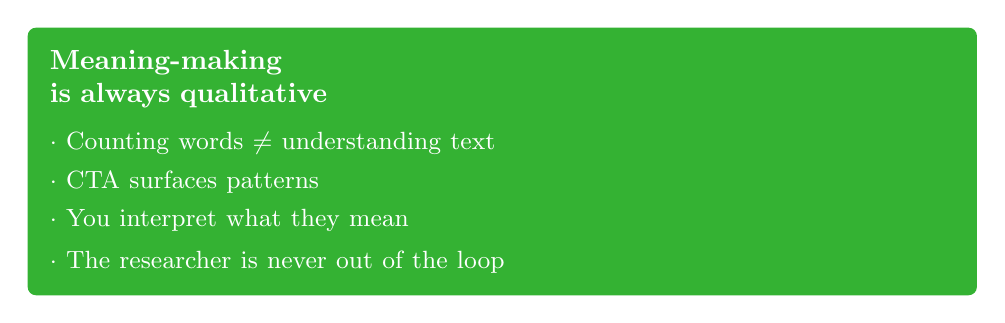
\begin{tikzpicture}
      \node[fill=wurgreen, rounded corners=3pt,
            inner xsep=8pt, inner ysep=8pt, text width=\columnwidth-18pt]{%
        \textcolor{white}{\textbf{Meaning-making\\is always qualitative}}\\[6pt]
        {\small\textcolor{white}{
        $\cdot$ Counting words $\neq$ understanding text\\[3pt]
        $\cdot$ CTA surfaces patterns\\[3pt]
        $\cdot$ You interpret what they mean\\[3pt]
        $\cdot$ The researcher is never out of the loop}}};
    \end{tikzpicture}
\end{columns}

\bigskip
{\small\textcolor{midgray}{\textit{Think of CTA as a tool, not a paradigm --- it serves your research question, whatever that is.}}}
\end{frame}

% ── SLIDE 6: Why care? ───────────────────────────────────────────────────────
\begin{frame}{Why Should You Care?}
{\small\textcolor{midgray}{Research that would be impossible --- or take years --- without computation:}}

\bigskip
\begin{columns}[t]
  \column{0.48\textwidth}
    \begin{tikzpicture}
      \node[fill=lightgreen, draw=wurgreen, rounded corners=3pt,
            inner xsep=8pt, inner ysep=7pt, text width=\columnwidth-18pt]{%
        \textcolor{wurgreen}{\faNewspaper}\enspace
        {\small Analyzing 100,000 news articles to track how migration framing shifts over time}};
    \end{tikzpicture}

    \medskip
    \begin{tikzpicture}
      \node[fill=lightgreen, draw=wurgreen, rounded corners=3pt,
            inner xsep=8pt, inner ysep=7pt, text width=\columnwidth-18pt]{%
        \textcolor{wurgreen}{\faTwitter}\enspace
        {\small Classifying sentiment in millions of tweets after a political crisis}};
    \end{tikzpicture}

  \column{0.48\textwidth}
    \begin{tikzpicture}
      \node[fill=lightgreen, draw=wurgreen, rounded corners=3pt,
            inner xsep=8pt, inner ysep=7pt, text width=\columnwidth-18pt]{%
        \textcolor{wurgreen}{\faScroll}\enspace
        {\small Comparing parliamentary speeches across 20 years and 5 countries}};
    \end{tikzpicture}

    \medskip
    \begin{tikzpicture}
      \node[fill=lightgreen, draw=wurgreen, rounded corners=3pt,
            inner xsep=8pt, inner ysep=7pt, text width=\columnwidth-18pt]{%
        \textcolor{wurgreen}{\faComments}\enspace
        {\small Making sense of thousands of open-ended survey responses without losing the nuance}};
    \end{tikzpicture}
\end{columns}
\end{frame}

% ── SLIDE 7: What for your research? ────────────────────────────────────────
\begin{frame}{What Could This Mean for Your Research?}
\vspace{0.1cm}
{\small\textit{Think about your own work for a moment\ldots}}

\bigskip

\begin{tikzpicture}
  \node[fill=lightgray, rounded corners=3pt,
        inner xsep=10pt, inner ysep=8pt, text width=\textwidth-22pt]{%
    \textcolor{wurgreen}{\faFolder}\enspace
    {\small What text data do you already have, or could realistically collect?}};
\end{tikzpicture}

\medskip

\begin{tikzpicture}
  \node[fill=lightgray, rounded corners=3pt,
        inner xsep=10pt, inner ysep=8pt, text width=\textwidth-22pt]{%
    \textcolor{wurgreen}{\faQuestion}\enspace
    {\small What research question could you explore if you could read 10{,}000 texts?}};
\end{tikzpicture}

\medskip
\begin{tikzpicture}
  \node[fill=lightgray, rounded corners=3pt,
        inner xsep=10pt, inner ysep=8pt, text width=\textwidth-22pt]{%
    \textcolor{wurgreen}{\faCog}\enspace
    {\small Where does analysis currently take the most time --- and could it be automated?}};
\end{tikzpicture}

\bigskip
{\small\textit{\textcolor{midgray}{\centering We'll come back to your answers throughout the week!}}}
\end{frame}

% ── SLIDE 8: Course overview ─────────────────────────────────────────────────
\begin{frame}{The Journey Ahead --- 4 Days}
\vspace{0.5cm}
\tikzset{daycard/.style={rounded corners=2pt, inner xsep=6pt, inner ysep=8pt,
         text width=3.1cm, minimum height=4.6cm, anchor=north west, align=left}}

\begin{tikzpicture}
  \node[daycard, fill=wurgreen] at (0,0) {%
    {\tiny\textcolor{white}{DAY 1}}\\[2pt]%
    {\scriptsize\bfseries\textcolor{white}{Text Data in Python}}\\[6pt]%
    {\tiny\textcolor{white}{$\cdot$ Python recap}}\\[2pt]%
    {\tiny\textcolor{white}{$\cdot$ Loading \& exploring text}}\\[2pt]%
    {\tiny\textcolor{white}{$\cdot$ Tokenization}}%
  };
  \node[daycard, fill=darkgreen] at (3.35,0) {%
    {\tiny\textcolor{white}{DAY 2}}\\[2pt]%
    {\scriptsize\bfseries\textcolor{white}{Bag-of-Words}}\\[6pt]%
    {\tiny\textcolor{white}{$\cdot$ Word frequencies}}\\[2pt]%
    {\tiny\textcolor{white}{$\cdot$ TF-IDF}}\\[2pt]%
    {\tiny\textcolor{white}{$\cdot$ Topic modeling (LDA)}}%
  };
  \node[daycard, fill=bodytext] at (6.7,0) {%
    {\tiny\textcolor{midgray}{DAY 3}}\\[2pt]%
    {\scriptsize\bfseries\textcolor{white}{Static Embeddings}}\\[6pt]%
    {\tiny\textcolor{white}{$\cdot$ Word2Vec \& GloVe}}\\[2pt]%
    {\tiny\textcolor{white}{$\cdot$ Pre-trained models}}\\[2pt]%
    {\tiny\textcolor{white}{$\cdot$ Similarity \& viz.}}%
  };
  \node[daycard, fill=darknavy] at (10.05,0) {%
    {\tiny\textcolor{midgray}{DAY 4}}\\[2pt]%
    {\scriptsize\bfseries\textcolor{white}{Contextual Embeddings}}\\[6pt]%
    {\tiny\textcolor{white}{$\cdot$ Transformers \& BERT}}\\[2pt]%
    {\tiny\textcolor{white}{$\cdot$ HuggingFace}}\\[2pt]%
    {\tiny\textcolor{white}{$\cdot$ Your own data}}%
  };
\end{tikzpicture}
\end{frame}

% ── SLIDE 9: Practicalities ──────────────────────────────────────────────────
\begin{frame}{Practicalities}
\vspace{0.2cm}
\begin{columns}[t]
  \column{0.32\textwidth}
    \centering\textcolor{wurgreen}{\faClock}\\[4pt]
    \textbf{Schedule}\\[6pt]
    \begin{flushleft}
    {\small
      10:00 -- 12:30 \quad Morning\\[3pt]
      12:30 -- 13:30 \quad Lunch\\[3pt]
      13:30 -- 16:00 \quad Afternoon
    }
    \end{flushleft}

  \column{0.32\textwidth}
    \centering\textcolor{wurgreen}{\faPython}\\[4pt]
    \textbf{Tools}\\[6pt]
    \begin{flushleft}
    {\small
      Google Colab (browser-based,\\no installation needed!)\\[3pt]
      NLTK, scikit-learn,\\gensim, transformers\\[3pt]
      \textit{Links to notebooks provided}
    }
    \end{flushleft}

  \column{0.32\textwidth}
    \centering\textcolor{wurgreen}{\faBook}\\[4pt]
    \textbf{Prerequisites}\\[6pt]
    \begin{flushleft}
    {\small
      Basic Python\\(DataCamp level)\\[3pt]
      No prior CTA knowledge needed --- we start from scratch
    }
    \end{flushleft}
\end{columns}
\end{frame}

% ── SLIDE 10: Let's go ───────────────────────────────────────────────────────
{
\setbeamertemplate{footline}{}
\begin{frame}[plain]
  \begin{tikzpicture}[remember picture, overlay]
    \fill[wurgreen] (current page.south west) rectangle (current page.north east);
    \fill[darknavy] (current page.south west) rectangle
      ([xshift=0.45cm]current page.north west);
    \node[text=white, font=\Huge\bfseries, anchor=west]
      at ([xshift=1.1cm, yshift=0.5cm]current page.west)
      {Let's get started! \faRocket};
    \node[text=darknavy, font=\large, anchor=west]
      at ([xshift=1.1cm, yshift=-0.6cm]current page.west)
      {Any questions before we dive into Python and text data?};
  \end{tikzpicture}
\end{frame}
}

\end{document}
